\documentclass[12pt,letterpaper,noanswers]{exam}
\usepackage[usenames,dvipsnames,svgnames,table]{xcolor}
\usepackage[margin=0.9in]{geometry}
\renewcommand{\familydefault}{\sfdefault}
\usepackage{multicol}
\pagestyle{head}
\header{AM 111 Class 17}{}{Numerical differentiation, p.\thepage}
\runningheadrule
\headrule
\usepackage{siunitx}
\usepackage{graphicx} % more modern
\usepackage{amsmath} 
\usepackage{amssymb} 
\usepackage{hyperref}
\usepackage{tcolorbox}
\usepackage{enumitem}
\def\mbf{\mathbf}
\newcommand{\vc}[1]{\boldsymbol{#1}}
\def\dsst{\displaystyle}
\DeclareMathOperator*{\argmin}{arg\,min} % thin space, limits underneath in displays


\begin{document}
 \pdfpageheight 11in 
  \pdfpagewidth 8.5in

\noindent 

\section*{Preliminaries}

\begin{itemize}
\itemsep0pt
\item The problem set and project proposal are due on Friday.
\item There will be a skill check in class during the next class.  The problem info is below.
\end{itemize}


\noindent\textbf{Big picture}

Today: Approximating $\frac{df}{dx}$ at a point $x_0$.

\vspace{0.2cm}
\hrule
\vspace{0.2cm}

\noindent \textbf{Skill check practice}

Let $f(x) = x^3 - 3x$.  Write an expression for $f'(x)$ approximated using central differences at $x_0 = 2.0$ with $h = 0.01$.

\emph{You will be asked for one of forward differences, central differences, or backward differences.}


\vspace{0.2cm}
\hrule
\vspace{0.2cm}

\noindent \textbf{Skill check solution}
 The formula is $(f(x+h) - f(x-h))/(2h)$ so $\dfrac{2.01^3-3*2.01 - 2^3+3*2}{0.02}$.


\vspace{0.2cm}
\hrule
\vspace{0.2cm}



\section*{Numerical differentiation}




\subsection*{Symbolic derivatives}
\begin{tcolorbox}

(Humpherys Volume 1 Lab 8)

To take the derivatives of a function known in closed form, try symbolic differentiation.  In Python the package is \texttt{sympy}.
\begin{verbatim}
import sympy as sy
x = sy.symbols('x')
# Differentiate x^3 + x with respect to x:
sy.diff(x**3 + x, x)
\end{verbatim}

You can evaluate the output of \texttt{sy.diff} at a point $x_0$ to find a value for $f'(x_0)$.
\end{tcolorbox}

\subsection*{Taylor's Remainder Theorem}


\subsection*{Approximating derivatives via finite differences}

\begin{enumerate}[resume=classQ]
\item Rearrange the expression 
\[f(x+h) = f(x) + hf'(x) + \frac{1}{2}h^2 f''(c)\] where $x< c< x+h$
from Taylor's theorem to isolate $f'(x)$ on the left hand side.
\vspace{1in}

\end{enumerate}


\begin{enumerate}[resume=classQ]
\item The three point \textbf{centered difference} formula is given by $f'(x) \approx \dfrac{f(x+h)-f(x-h)}{2h}$.  We want to find the truncation error.
\begin{parts}
\item Taylor expand $f(x+h)$ and $f(x-h)$ to second order (with a third order error term).  When you calculate $\dfrac{f(x+h)-f(x-h)}{2h}$ what do you find?
\vspace{1in}

\item Find $n$ such that $f'(x) = \dfrac{f(x+h)-f(x-h)}{2h} + h^n k$ where $k$ is a constant.
\vspace{1cm}

\end{parts}
\end{enumerate}

\begin{enumerate}[resume=classQ]
\item Now we'll look at rounding error.  Let the floating point version of $f(x+h)$ be $\hat{f}(x+h)$.

$\hat{f}(x+h) = f(x+h) + \epsilon_1$ where $\vert \epsilon_1\vert \approx \epsilon_{\text{mach}}$.

$\hat{f}(x) = f(x) + \epsilon_2$ where $\vert \epsilon_2\vert \approx \epsilon_{\text{mach}}$.

$\hat{f}(x-h) = f(x-h) + \epsilon_3$ where $\vert \epsilon_3\vert \approx \epsilon_{\text{mach}}$.

\begin{parts}
\item Compare $\dfrac{\hat{f}(x+h) - \hat{f}(x)}{h}$ to $\dfrac{f(x+h) - f(x)}{h}$.  What is the maximum error due to rounding?
\vspace{1in}

\item Sum the truncation error and the rounding error to generate an error estimate for $f'(x)$ when calculated using forward differences.
\vspace{1cm}


\item Do the same for $f'(x)$ when calculated using central differences.
\vspace{1in}

\end{parts}


\end{enumerate}

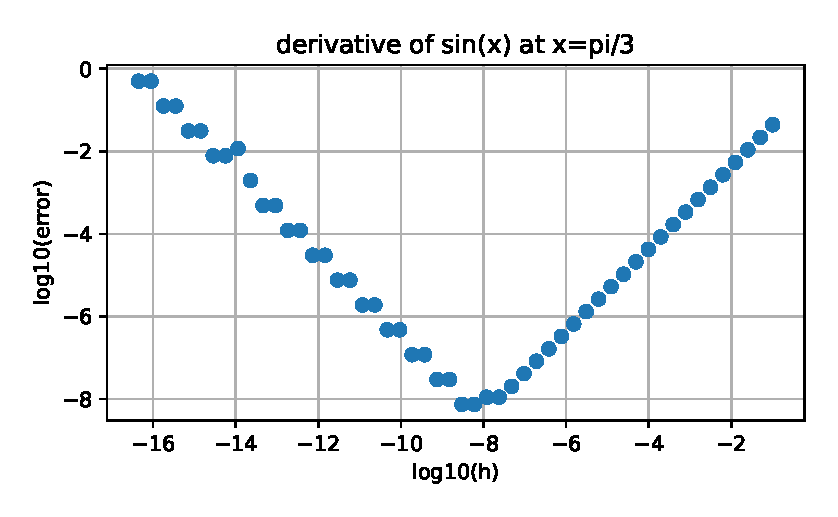
\includegraphics[width=0.5\textwidth]{img/Class11sinforward.eps}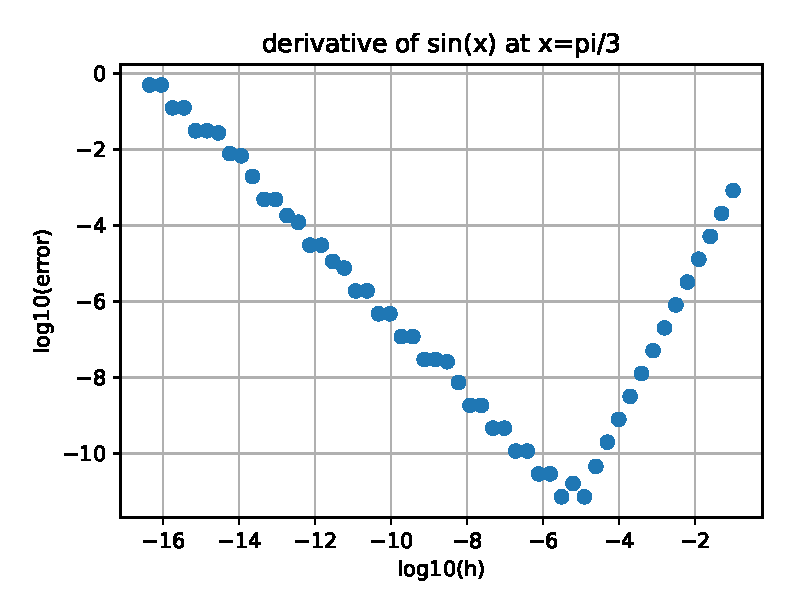
\includegraphics[width=0.45\textwidth]{img/Class11sincentral.eps}



\begin{enumerate}[resume=classQ]
\item Examine the log-log plot of error shown on the left above.
\begin{parts}
\item The error function is approximately two straight lines on the log-log plot.  Which part is dominated by truncation error and which by rounding error?
\vspace{1cm}

\item Using the grid, approximate the two slopes.
\vspace{1cm}

\item Which error function do they match?  Take the log of both sides of your error function to identify the expected slopes.
\vspace{0.5in}

\item Answer the same questions for the plot shown on the right above.
\vspace{0.5in}

\end{parts}

\end{enumerate}



\begin{enumerate}[resume=classQ]
\item For each error function, find the value of $h$, in terms of machine epsilon, that minimizes the total error.

Compare your findings to the plots.
\vspace{1in}
\end{enumerate}

\subsection*{Approximating a derivative from data}

\begin{enumerate}[resume=classQ]
\item Assume the maximum measurement error is $\delta \vert f(x_i)\vert$.  Replace $\epsilon_{\text{mach}}$ in your rounding error calculation with $\delta \vert f(x_i)\vert$ to find an expression for the maximum error due to measurement error.

\vspace{1in}


%then it propagates to the derivative as $\dfrac{\delta}{h}(\vert f(x_{i+1})\vert + \vert f(x_{i})\vert)$ where $h = x_{i+1}-x_i$.
\end{enumerate}


\begin{enumerate}[resume=classQ]
\item Consider the three functions plotted on the left below.  
\begin{parts}
\item What is the largest difference in $y$ that occurs between any two functions?  What is the smallest difference?
\vspace{1cm}
\item Find the derivative of each function.
\vspace{1in}
\item If the true function were $f(x) = x$, but your measurement method added high frequency noise, so that the data looked exactly like $x + 0.01\sin(100x)$, what is the maximum error you would see in the derivative?
\vspace{1cm}

\item Thinking of your derivative as your output (forward error) and your measurements as your input (backward error), create an estimate of an absolute condition number.
\vspace{1cm}
\end{parts}



\end{enumerate}

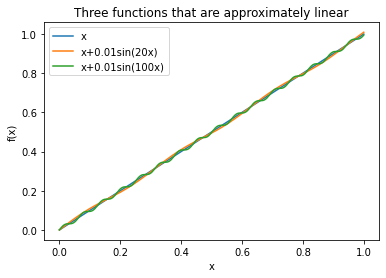
\includegraphics[width = 0.45\linewidth]{img/Class11lines.png}
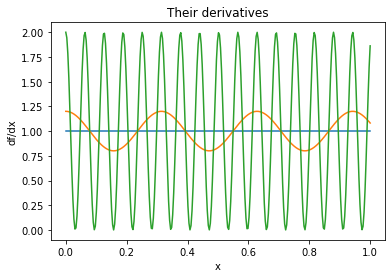
\includegraphics[width = 0.45\linewidth]{img/Class11linederiv.png}

% \begin{enumerate}[resume=classQ]
% \item 
% \end{enumerate}


\end{document}